%% ====== Classe du document ============================================
\documentclass[10pt,a4paper]{article}
%\usepackage[left=1.5cm,right=1.5cm,top=2cm,bottom=2cm]{geometry}

%% ====== Francisation ==================================================
\usepackage[french]{babel}
\usepackage[T1]{fontenc}
\usepackage[utf8]{inputenc}
\usepackage{textcomp}

%% ====== Personnalisation ============================================
\usepackage{fancyhdr}
	\lhead{}
	\chead{Projet MDMA - Rapport L2}
	\rhead{M1 IF 2012-2013}
	\renewcommand{\headrulewidth}{0.3pt}
	\renewcommand{\footrulewidth}{0.3pt}
	\lfoot {}
	\cfoot {- \thepage -}
	\rfoot {}
	\pagestyle{fancy}
\title{Projet MDMA - Rapport L2}
\author{}
\date{}

\usepackage{hyperref}

%% ====== Packages pour le texte ========================================
%\usepackage{soul}
%\usepackage[normalem]{ulem}
%\usepackage{fancybox}
%\usepackage{moreverb}
%\usepackage[table]{xcolor}
%% ====== Packages pour les dessins =====================================
\usepackage{float}
\usepackage{graphicx}
%\usepackage{multicol}
%\usepackage{multirow}
%\usepackage{tikz}
%\usepackage{lmodern}
\usepackage{pict2e}

%% ====== Packages pour les maths =======================================
%\usepackage{amsmath}
%\usepackage{amssymb}
%\usepackage{mathrsfs}
%\usepackage{bussproofs}
%\usepackage[ruled,vlined,french]{algorithm2e}

%%% francisation des algorithmes

%\usepackage[squaren,Gray]{SIunits}
%% ====== Reglages generaux =============================================

\usepackage{titlesec}
	\titleformat{\section}[frame]
	{\normalfont}
	{\filright
	\footnotesize
	\enspace Partie \thesection\enspace}
	{6pt}
	{\bfseries\filcenter}
	
	\titleformat{\subsection}[frame]
	{\normalfont}
	{\filright
	\footnotesize
	\enspace \thesubsection\enspace}
	{6pt}
	{\filcenter}
%	{\titlerule
%	\vspace{.8ex}%
%	\normalfont\itshape}
%	{\thesubsection.}{.5em}{}

	\titleformat{\subsubsection}
	{\titlerule
	\vspace{.8ex}%
	\normalfont\itshape}
	{}{.5em}{}

\titleformat{\chapter}[display]
	{\normalfont\bfseries\filcenter}
	{}
	{1ex}
	{\titlerule[2pt]
	\vspace{2ex}%
	\LARGE}
	[\vspace{1ex}%
	{\titlerule[2pt]}]
	
\parindent=10pt

%\usepackage{makeidx}
%\makeindex
%\newcommand\vect{\overrightarrow}

%\numberwithin{equation}{subsection}


\graphicspath{{img/}}

\usepackage[svgnames]{xcolor}
\usepackage{pgfgantt}


%% ================================================================
\begin{document}
\maketitle
%\tableofcontents
%% ================================================================
\paragraph{Coordinateurs :} Timothée Bernard, Louis Parlant
\paragraph{Membres du projet :} Hadrien Croubois, Henri Derycke, Gaëtan Gilbert, Semen Marchuk, Luc Rocher

\subsection*{Description détaillée}
\par Ce projet a pour but de mettre au point un contrôleur MIDI logiciel basé sur la reconnaissance de mouvements par webcam. Le MIDI est un protocole très utilisé pour piloter les synthétiseurs matériels tout comme les logiciels de musique assistée par ordinateur (MAO), devenu un standard depuis sa présentation en 1983 ; il permet d'échanger des messages simples sur trois octets qui sont interprétés comme des notes ou des changements de paramètre par les appareils connectés en sortie. Les contrôleurs MIDI sont quant à eux des dispositifs matériels ou logiciels émettant des signaux MIDI.

\par Un message MIDI possède toujours la forme suivante : un 0 suivi de trois bits déterminant le type de message (il y a huit types possibles, appelés "note off", "note on", "polyfonic aftertouch", "channel pressure", "program change", "control change", "pitch bending" et "system", bien que certains, comme "polyfonic aftertouch", soient beaucoup plus rarement utilisés que d'autres), de quatre bits déterminant le canal du message (un appareil ou un logiciel peut être configuré pour n'écouter que certains canaux), puis de deux octets commençant tous deux par un 1 et codant la valeur du message (la note jouée ainsi que son intensité pour un message de type "note on" par exemple). L'envoi de ce type de message est déjà implémenté par plusieurs bibliothèques ; nous commenceront pas nous intéresser à RtMidi\footnote{http://www.music.mcgill.ca/~gary/rtmidi/}.

\par Il existe de nombreux types de contrôleurs MIDI et les évolutions en la matière sont fréquentes : les constructeurs de ce type de matériel rivalisent d'originalité pour satisfaire les producteurs de musique électronique, du simple clavier-maître aux machines les plus élaborées (la série APC de Akai ou le Novation Launchpad en sont de bons exemples). Ce domaine est en plein essor, essentiellement grâce à la démocratisation de la MAO et de la popularité actuelle des musiques électroniques.

\par Notre approche consiste à développer un contrôleur MIDI d'un nouveau genre, sans aucune interaction physique avec du matériel. Le musicien veut avant tout diriger des séquenceurs et des instruments virtuels de manière intuitive. Il s'agit par exemple de lancer des clips audio, de jouer des notes via un synthétiseur ou une boîte à rythmes, ou encore de modifier les effets appliqués aux pistes gérées par différents logiciels de MAO.

\par Dans une optique d'ergonomie, pour garantir des manipulations fluides et naturelles, nous nous proposons de construire un contrôleur logiciel reconnaissant les mouvements du musicien à l'aide d’événements et de zones virtuelles pour simuler des claviers, des potentiomètres, des interrupteurs ou encore des \emph{faders}. Grâce à la \emph{webcam} de n'importe quel ordinateur, MDMA reconnaîtra des mouvements simples du musicien : mouvements de bras, positionnement des mains dans certaines zones, ouverture et fermeture des mains, frappe dans le vide, etc. Ensuite, il s'agira de traduire ces mouvements en commandes MIDI et de pouvoir les exporter vers un autre logiciel.

\subsubsection*{Public visé}

\par Ce projet vise donc avant tout le monde de la musique assistée par ordinateur, dans tous les styles possibles : tout synthétiseur virtuel pourra être contrôlé via MDMA, ainsi que des appareils physiques si l'ordinateur de l'utilisateur dispose d'une sortie MIDI, il pourra aussi être utilisé pour manipuler un logiciel de \emph{DJing}\footnote{activité consistant à mixer en temps réel différents morceaux en ajoutant éventuellement des effets audio} ou tout autre performance de musique électronique... Les possibilités sont multiples et c'est exactement aujourd'hui que ce domaine émet le plus de demandes et attend le plus d'innovations, en terme d'ergonomie notamment. Simple d'utilisation mais entièrement et aisément configurable, MDMA ciblera autant le novice en MAO  à la recherche d'un moyen ludique de contrôler ses logiciels que le musicien expérimenté ayant le besoin d'un outil naturel et cohérent lui permettant de produire de la musique sur scène à partir d'un ordinateur.

\subsubsection*{Réalisations logicielles}

\par A terme, ce projet se présentera sous la forme suivante.
A l'ouverture du logiciel MDMA, une fenêtre s'ouvre et propose de configurer le contrôleur. L'image acquise par la webcam est affichée, le musicien se voit bouger à l'écran et peut alors grâce à quelques outils simples dessiner diverses zones réactives autour de lui : des rectangles à l'intérieur desquels des actions particulières de l'utilisateur appelleront une fonction, des segments servant d'interrupteurs lorsqu'une main les traverse... On pourra alors décider de quels genres d'effets sont assignés à chaque zone, comme l'envoie de commandes, servant à simuler un \emph{fader} ou un \emph{pad x/y} par exemple. La configuration préliminaire se doit d'être maniable et facile à faire. Le musicien pourra utiliser des \emph{presets} standards ou créer et sauvegarder les siens. Le musicien a la possibilité de disposer de plusieurs onglets différents pendant une session, c'est à dire qu'il pourra construire trois configurations indépendantes utilisables en direct. Il peut naviguer de l'une à l'autre grâce à des commandes particulières dont l'activation est assignable aux zones décrites précédemment.

\par Une fois les zones réactives disposées et leurs fonctions choisies, l'utilisateur peut lancer MDMA et celui-ci commence à envoyer des signaux MIDI correspondant à chacun de ses mouvements. Dans le cas typique, il lance alors son séquenceur et peut assigner chacune des commandes MIDI à un événement. Par exemple, il associera les commandes d'un onglet à un gestionnaire de clips audio en utilisant ses zones réactives pour le lancement de boucles instrumentales, puis il utilisera un second onglet comme un \emph{sampler}, certains de ses mouvements correspondant alors à un petit échantillon musical (son de batterie, extrait vocal...), enfin un troisième onglet lui servirait à simuler une gamme de potentiomètres virtuels pour gérer des effets, la vitesse ou la hauteur des notes, etc.

\begin{figure}
	\begin{center}
		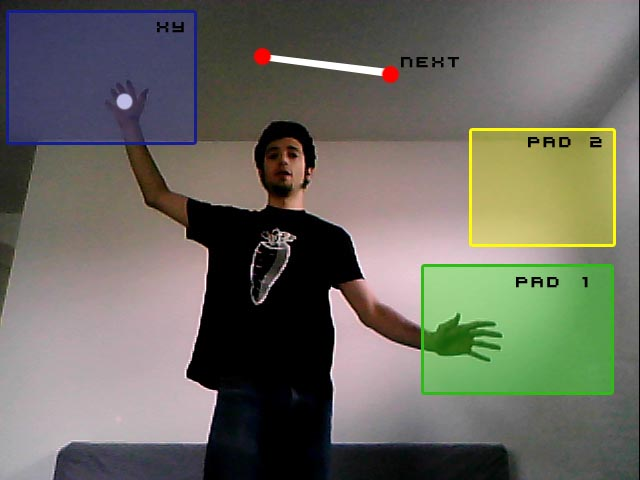
\includegraphics[width=5cm]{mdma1.jpg}
		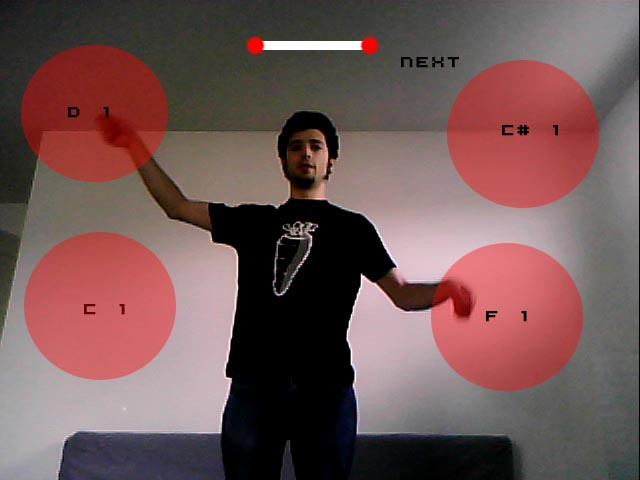
\includegraphics[width=5cm]{mdma2.jpg}
		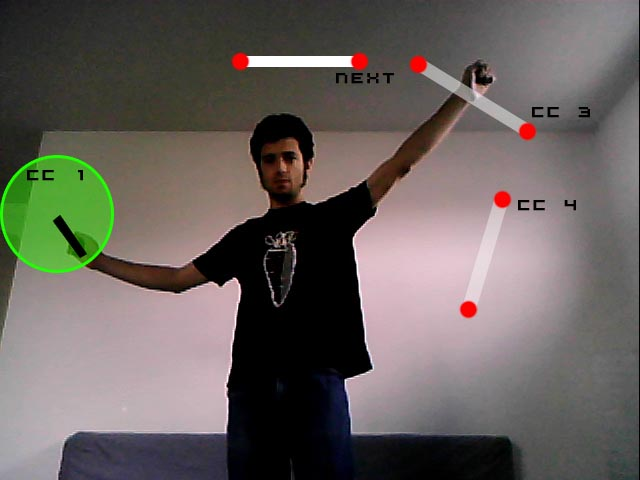
\includegraphics[width=5cm]{mdma3.jpg}
	\end{center}
	\caption{Exemple de ce à quoi devrait ressembler la fenêtre de visualisation}
\end{figure}

\subsubsection*{Choix d’implémentation \& fonctionnalités}

\par Concrètement, nous implémenterons cet outil en C++ en utilisant certaines bibliothèques adaptées parmi lesquels le framework Qt.
Qt est un framework multiplatforme disponible sous licence LGPL permettant la réalisation de fenêtres graphiques complètes ainsi que de nombreuses fonctionnalités telles que de puissants outils de multithreading et la possibilité de communiquer entre objets par le biais de signaux. Le caractère multiplatforme de Qt nous semble par ailleurs fondamental, en effet, compte tenu des supports utilisés en musique électronique, nous ne pouvons pas produire un logiciel seulement utilisable sous Linux, nous nous efforcerons donc de rendre notre programme disponible sous Windows, puis éventuellement dans un second temps Mac OS. Qt est par ailleurs très largement utilisé notament par Adobe, Google, Boeing et la Nasa.

\par La capture et l'analyse d'image se fera quand à elle en utilisant OpenCV, qui permet de repérer assez facilement des mouvements des mains. Nous aurons donc accès aux coordonnées de chaque main qui nous permettront de déterminer leur vitesse, leur accélération, ainsi que leur position par rapport à chaque zone réactive durant les mouvements du musiciens. Cela nous permettra de détecter plusieurs types de comportements :
\begin{description}

	\item[Entrée et sortie dans une zone] On peut grâce à la position de la main calculer si elle est dans une zone précédemment délimitée. On sait alors que toute action que l'utilisateur y fera sera à lier aux événements de cette zone.
	\item[Franchissement de segment] On pourra utiliser des segments que le musicien franchira avec ses mains pour s'en servir comme d'un interrupteur. Calculer à quel moment le franchissement a lieu, et éventuellement à quelle vitesse, ne posera pas de problème.
	\item[Ouverture et fermeture des mains] Si l'utilisateur ouvre ou ferme sa main dans une zone particulière, nous créerons un événement associé à cette action afin de pouvoir l'assigner plus tard à, par exemple, un lancement de clip. Cela permettrait aussi au musicien de saisir des objets virtuels et de les déplacer une fois que sa main s'est refermée dessus : des clips, un curseur sur un pad, un \emph{fader}...
	\item[Frappe] Nous tenterons de détecter le plus précisément possible les mouvements de frappe, comparables à ceux d'un batteur. Pour cela, nous nous baserons sur l’accélération : la variation brutale de la vitesse d'une main (si elle change de sens en un laps de temps très court par exemple) devrait bien caractériser ce type de mouvement.
\end{description}

\par L'analyse de ces comportements sera possible grâce aux fonctionnalités très riches d'OpenCV framework. Étant capable d'automatiser des opérations comme des détections de limites, des analyses des gradients, des soustractions d'images pour trouver les différences, des corrections des caractéristiques générales de l'image (luminosité, contraste), et possédant les instruments pour réaliser effectivement les opérations vectorielles, OpenCV nous aidera à éviter la réalisation d'instruments standards de traitement de l'image. Un grand atout pour le projet est l'existence d'implémentations renforcées par les GPU.
Plus précisément, le MDMA analysera ces différents mouvements grâce à OpenCV et créera des événements associés.
% gestion d'événement, Qt et toussa
Le logiciel exportera finalement ces événements sous forme de messages MIDI. Nous n'utiliserons que deux types de messages : les \emph{note on}, pour transmettre des notes en encodant leur hauteur et leur vélocité, et les \emph{control change}, qui permettent de modifier certains paramètres du logiciel en sortie (en simulant la rotation d'un potentiomètre par exemple). Ces derniers devront transmettre un numéro de contrôleur (i.e. un identifiant auquel le logiciel en sortie peut assigner un certain comportement) et la valeur qu'on lui donne. Pour que MDMA soit pleinement et facilement utilisable, il faut être capable de créer un port MIDI out virtuel auquel les autres logiciels peuvent se connecter. À première vue, RtMidi ne semble pas être capable de faire cela pour les systèmes Windows, il sera peut-être nécessaire de se tourner vers d'autres logiciels tels que loopMIDI\footnote{http://www.tobias-erichsen.de/loopMIDI.html} ou LoopBe1\footnote{http://www.nerds.de/en/loopbe1.html}.

\subsubsection*{L'équipe}

\par L'équipe MDMA est composée de sept personnes : Timothée Bernard, Hadrien Croubois, Henri Derycke, Gaëtan Gilbert, Semen Marchuk, Louis Parlant et Luc Rocher.
\par Tout au long du développement Luc dirigera la communication du projet (interne et externe) avec l'aide d'Hadrien et de Timothée ; il s'agirait notamment de présenter ce projet aux milieux de la musique assistée par ordinateur. Les trois premières semaines Louis et Timothée dirigeront l'intégralité de l'équipe dans un workpackage visant à déterminer clairement les  spécifications de MDMA. Dès que celles-ci commenceront à être  suffisament clarifiées, des groupes dirigés respectivement par Gaëtan et Semen s'occuperont de l'interface Midi (i.e. la sortie du logiciel) et de l'interface OpenCV (récupération et analyse du flux vidéo). Lorsque les spécifications auront été données, Hadrien pourra commencer à  travailler sur l'aspect graphique de MDMA et Henri cherchera des solutions algorithmiques pour détecter et gérer les évènements correspondant aux mouvements de l'utilisateur. S'ensuivra à partir de mi-novembre une phase d'intégration, dirigée par Hadrien, visant à  vérifier et corriger l'interopérabilité des différents composants logiciels précédemment codés, et de test, dirigé par Timothée, pour la rercherche de bugs, l'ergonomie et la conformité aux spécifications initiales, aboutissant si tout fonctionne comme prévu à la mise au point de différentes versions préliminaires avant la fin du projet.
\par L'avancée progressive du développement sera mise en commun à l'aide d'un dépôt GIT d'ores et déjà mise en place.\footnote{https://github.com/Amxx/MDMA}
\par Certaines améliorations seront possibles, et ce projet pourra perdurer si on nous en donne l'opportunité. Nous penserions par exemple à réaliser un MDMA multi-plateformes, utilisable sous Windows, Mac OS ou distributions Linux, ou encore à affiner l'analyse des mouvements en utilisant une \emph{kinect}...

\subsection*{Workpackages}
\begin{ganttchart}%
[
x unit=0.8cm, y unit title=0.4cm,y unit chart=0.5cm,
vgrid={*1{RoyalBlue!50,dashed}}, hgrid=false,
title/.style={draw=none, fill=RoyalBlue!50!black},
title label font=\sffamily\bfseries\color{white},
title label anchor/.style={below=-1.6ex},
title left shift=.02,
title right shift=-.02,
title height=1,
group/.style={draw=black, fill=RoyalBlue!50!black},
group height=.3,
group peaks={.1}{.2}{.2},
bar/.style={draw=RoyalBlue!50!black, fill=SteelBlue!75, rounded corners=.5mm},
bar height=.6,
bar label font=\normalsize\color{black!50},
progress label anchor/.style={left=0cm},
incomplete/.style={fill=SteelBlue!25},
link/.style={thick, ->, RoyalBlue, rounded corners=.5mm}
]{12}
		
\gantttitle{Oct}{4}\gantttitle{Nov}{4}\gantttitle{Dec}{4}\\
\ganttbar[name=spec]{[Timothée, Louis] Spécifications}{1}{3}\\
\ganttbar[name=desi]{[Hadrien] Design interface}{4}{6}\\
\ganttbar[name=midi]{[Gaëtan] Interface Midi}{2}{5}\\
\ganttbar[name=open]{[Semen] Interface openCV}{2}{5}\\
\ganttbar[name=even]{[Henri] Caractérisation des événements}{4}{7}\\
\ganttbar[name=inte]{[Hadrien] Intégration}{7}{12}\\
\ganttbar[name=test]{[Timothée] Testing}{7}{12}\\
\ganttbar[name=comm]{[Luc] Communication}{1}{12}\\
\end{ganttchart}

\begin{description}
\item[Spécifications] \emph{Timothée \& Louis} + tout le monde
\item[Design graphique] \emph{Hadrien}, Luc 10\%
\item[Interface MIDI] \emph{Gaëtan}, Timothée, Louis 100\%
\item[Interface OpenCV] \emph{Semen}, Henri, Hadrien
	\par Détection de mouvements de la main (ouverture/fermeture, accélération, etc)
\item[Gestion des événements] \emph{Henri 60\%}, Semen 40\%, Hadrien
	\par Caractérisation des objets « zones »
\item[Communication] \emph{Luc 90\%}, Timothée, Hadrien 5\%
	\par Gestion du site Internet
	\par Communication extérieure
\item[Intégration \& test] \emph{Hadrien \& Louis 100\%}
\end{description}



%% ===================================================================
\end{document}
